%!TEX root = ../thesis.tex

\chapter{Anforderungsanalyse} % (fold)
\label{cha:anforderungsanalyse}

\todo{\small{Hier fehlt ein Anfang}}

\begin{figure}[ht]
     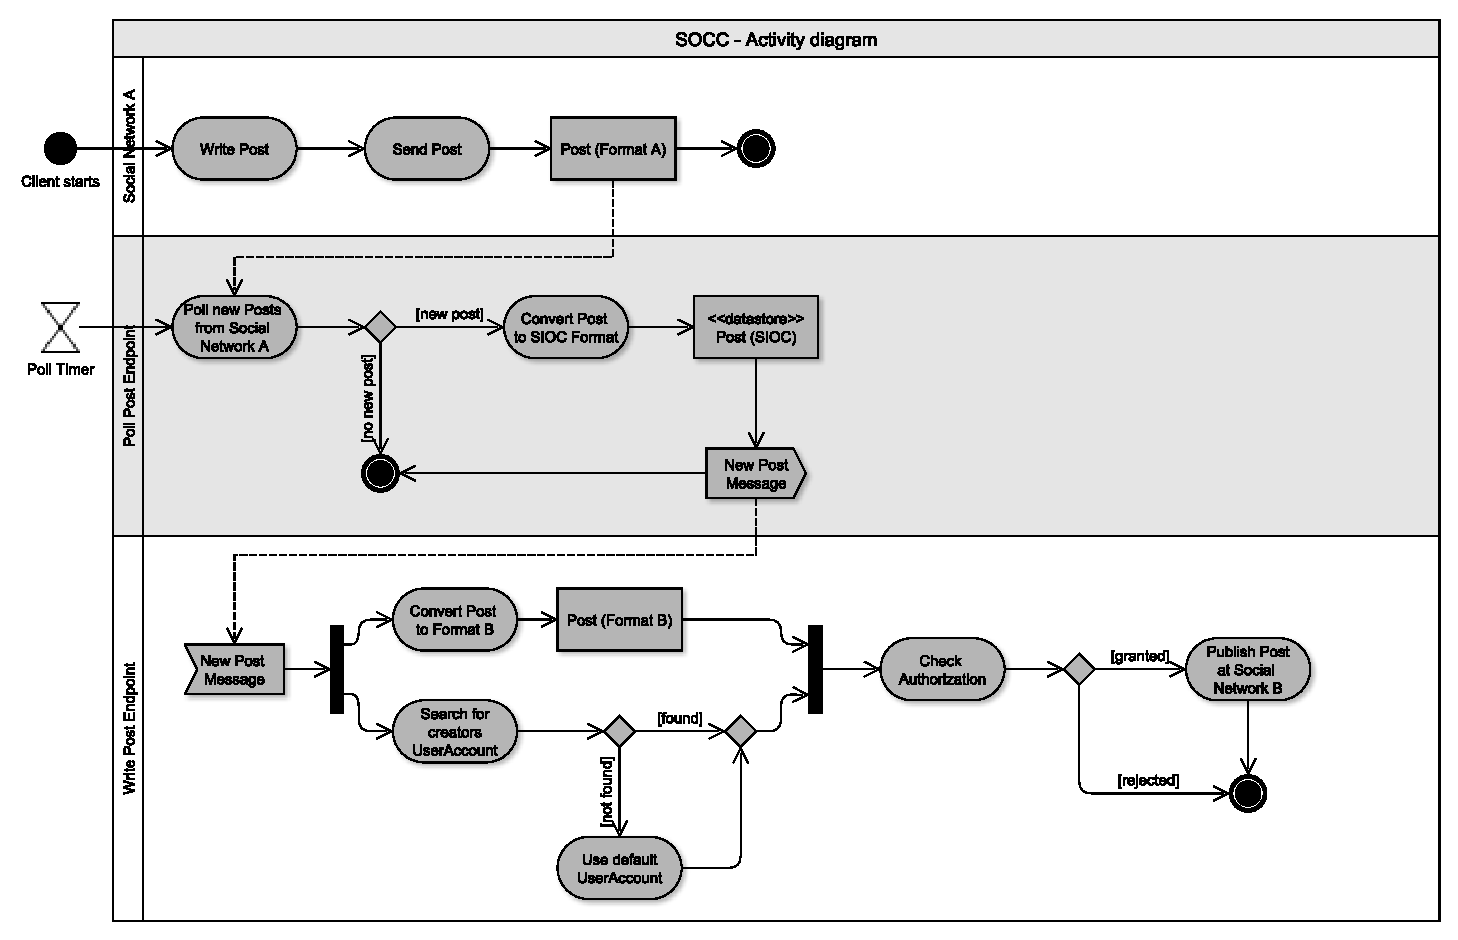
\includegraphics[
        width=\textwidth,
        keepaspectratio=true,
        clip=true,
        trim= 0 338 0 27
    ]{assets/images/activitydiagram_post_as_user_check_authorization.pdf}
    \caption{Benutzer erstellt einen Beitrag im sozialen Netzwerk A.}
    \label{fig:beutzer_erstellt_beitrag_a}
\end{figure}

Soziale Netzwerk A speichert die Daten der Nachricht in sein eigens Format A. Um diese Beiträge in das soziale Netzwerk B transferieren zu können, müssen zuerst die Daten über eine API von den Servern des sozialen Netzwerks A herunter laden. Da in der Regel nicht automatisch bekannt ist, wann eine neue Nachricht vorhanden ist, müssen die Server in zeitlichen Abständen abgefragt werden und die zurückgelieferten Daten nach neuen Beiträge durchsucht werden. Wurden neue Beiträge gefunden können diese nicht direkt an das soziale Netzwerk B geschickt werden, da sich diese in der Regel im verwendeten Format unterscheiden. Die einfachste Möglichkeit wäre nun die Daten von Format A nach Format B zu konvertieren. Bei zwei Netzen ist dies noch sehr einfach. Es müsste lediglich nur ein Konverter von A nach B und einer von B nach A implementiert werden. Kämme nun ein drittes Netzwerk C hinzu, wären sechs Konverter nötig (A $ \Rightarrow $ B, A $ \Rightarrow$  C, B $ \Rightarrow $ A, B $ \Rightarrow $ C, C $ \Rightarrow $ A und C $ \Rightarrow $ B). Nimmt man an $n_{sn}$ sei eine beliebige Anzahl sozialer Netzwerke, entspricht die Anzahl der Konverter $ n_{k1}= n_{sn}*(n_{sn}-1) $, da für jedes Netzwerk ein Konverter in alle anderen Netzwerke nötig wird. Aber auch die Konverter selber sind eine Herausforderung für sich. Nicht alle Formate sind gleich aufgebaut. Im einfachsten Fall unterscheiden sich die einzelnen Daten, aber ist es auch möglich das ein Netzwerk die Features eines Anderen nicht oder in einer abgewandelten Form anbietet. Als Beispiel wäre die Bewertung einzelner Beträge zu nennen. Ein Netzwerk nutzt hier einen, oft anzutreffenden, null bis fünf Sterne Bereiche, ein Anderes setzt auf positive und negative Bewertungen.

\medskip

Eine elegantere Methode, welche sowohl das Problem mit der starken Zunahme an Konvertern als auch der ähnlichen beziehungsweise unterschiedlichen Features lösen könnte, wäre die Einführung eines Zwischenformates. Alle anfallenden Daten würden erst einmal in dieses Zwischenformat und später in das entsprechende Zielformat konvertiert. Dadurch müssten für jedes neue soziale Netzwerk zwei Konverter, für das Schreiben und Lesen dieses Zwischenformates, implementiert werden. Die Anzahl an Konvertern bezieht sich dem zufolge auf $ n_{k2} = n_{sb} * 2 $. Nachteile hätte dieser Ansatz nur für $ n_{sn}=2 $ und $ n_{sn}=3$ , da in diesen Fällen mehr beziehungsweise gleich viele Konverter gegenüber der ersten Methode nötig wären. Aber schön für geringfügig höhere Werte sinkt die Anzahl der Konverter signifikant. Für $ n_{sn} = 4 $ wären es $ n{k2} = 8 $ statt $ n{k1} = 12 $ und für $ n_{sn} = 5 $ ergibt sich $ n{k2} = 10 $ statt $ n{k1} = 20 $ Konvertern. Demzufolge verringert sich auch der Implementierungsaufwand wenn mehrere Netzwerke unterstützt werden sollen.


\begin{figure}[h]
     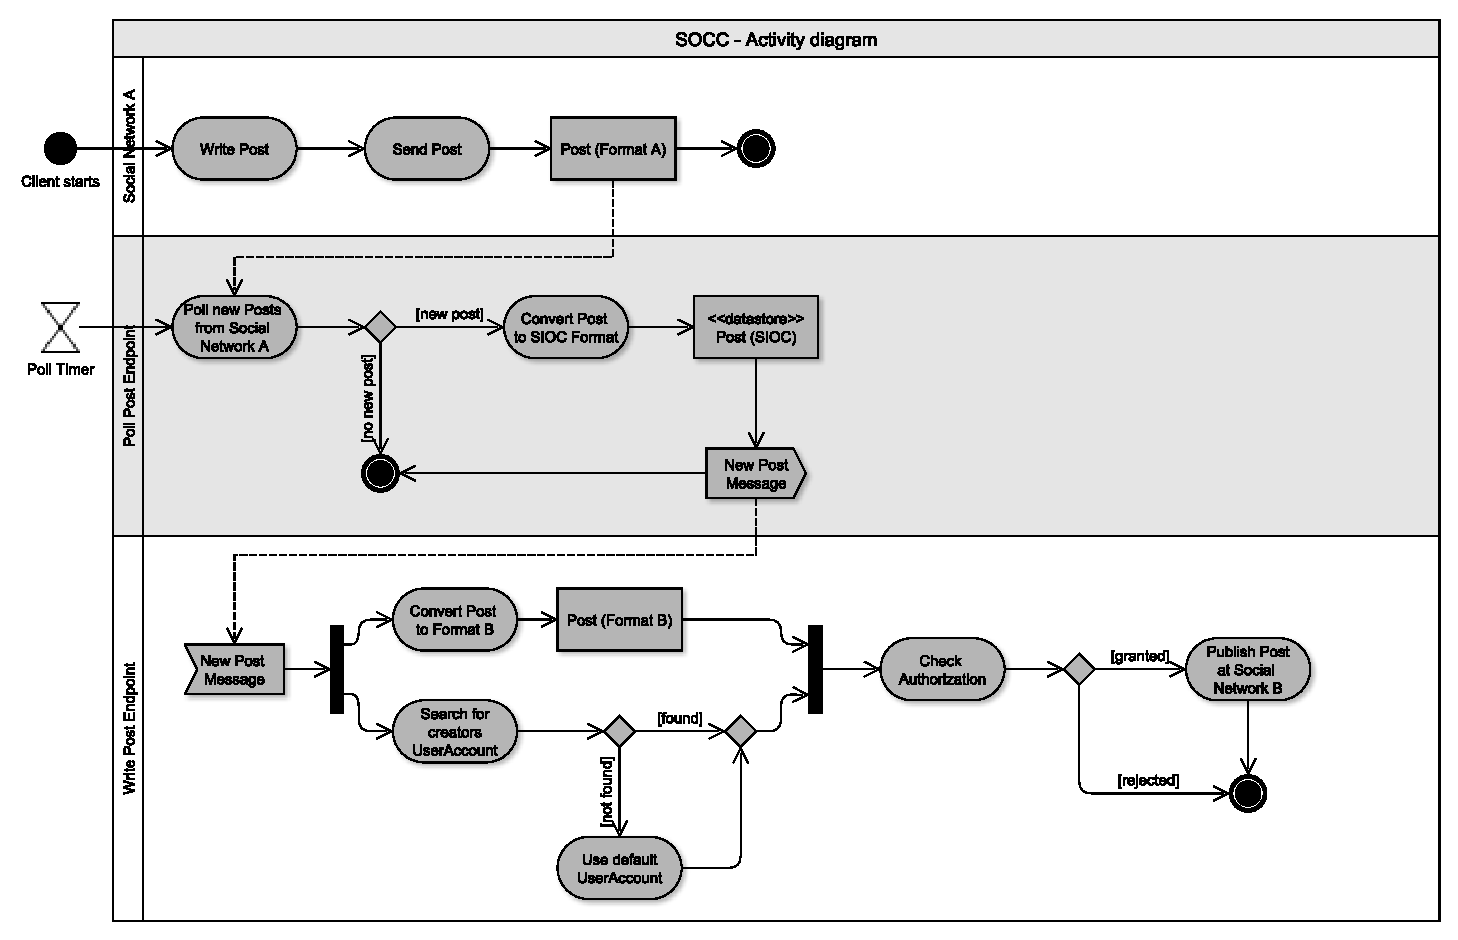
\includegraphics[
        width=\textwidth,
        keepaspectratio=true,
        clip=true,
        trim= 0 193 0 113
    ]{assets/images/activitydiagram_post_as_user_check_authorization.pdf}
    \caption{
        Lesen des erstellten Beitrags und konvertieren in das Zwischenformat.
    }
    \label{fig:lesen_von_beitrag_und_convertieren}
\end{figure}


Liegen nun alle Daten in diesem Zwischenformat können diese an einen zentralen Ort gespeichert werden. So ist es möglich diese Daten für die verschiedensten Zwecke weiter zu verarbeiten. Die Suche nach ähnlichen oder inhaltlich zusammenhängenden Beiträgen aus verschieden Quellen. Durch das gemeinsame Format ist dies  einfacher möglich als sich erst mit den unterschiedlichen Formaten der einzelnen Quellen auseinandersetzen zu müssen.

\medskip

Da mit diesem Projekt auch eine automatische Synchronisation neuer Beträge zwischen unterschiedlichen sozialen Netzwerken ermöglicht werden soll, muss das Eintreffen eines neuen Betrags an die entsprechenden Stellen weitergereicht werden. Da dieser Zeitpunkt nicht im Vorneherein bekannt ist würde sich hier ein Event-basierter Ansatz anbieten. So entsteht eine zeitliche Entkopplung des Lesens und Schreibens von Beträgen. Der Einsatz eines \enquote{Publish-Subscribe}-Mechanismus wäre hier ebenfalls von großen Vorteil, da so die Beträge eines sozialen Netzwerkes mit mehreren Synchronisiert werden kann. 

\medskip

Wurde nun ein Event, dass ein neuer Beitrag gelesen wurde, abgeschickt wird dieser über den besagten \enquote{Publish-Subscribe}-Mechanismus an alle dadurch verbundenen Endstellen weitergeleitet. Dieses konvertieren nun den Beitrag in das entsprechende Format des soziale Netzwerks und holen sich alle nötigen Information um diesen dort hin zuschicken. Eine wünschenswerte Erweiterung hierbei wäre \todo{Quelle suchen}, wenn der so geschriebene Beitrag dann so erscheinen würde, als hätte der Autor des ursprünglichen Beitrags ihn selber geschrieben. Hierzu müssten die einzelnen Benutzer das System, zum Beispiel durch das hinterlegen von Access Token\footnote{\url{http://oauth.net/}} oder anderen Authentifizierungsparameter, autorisieren in ihren Namen Nachrichten zu schreiben. Diese könnten dann anhand der Benutzerkennung herausgesucht und benutzt werden. 

\begin{figure}[h]
     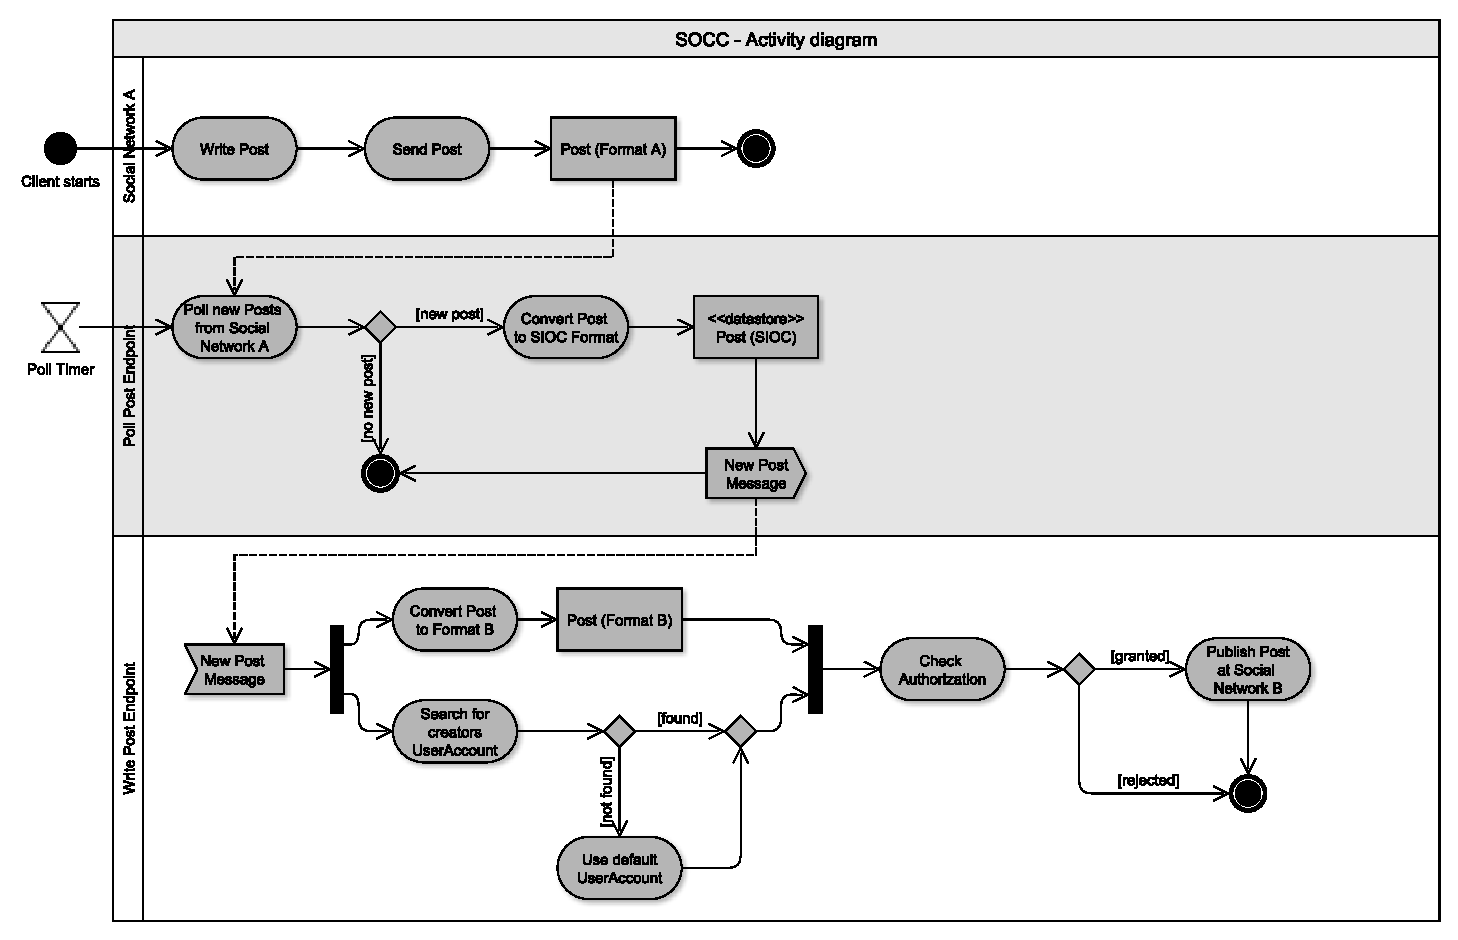
\includegraphics[
        width=\textwidth,
        keepaspectratio=true,
        clip=true,
        trim= 0 0 0 257
    ]{assets/images/activitydiagram_post_as_user_check_authorization.pdf}
    \caption{
        Konvertierten des Beitrags in das Format B und schreiben in das soziale Netzwerk B
    }
    \label{fig:konvertieren_formatb_und_schreiben}
\end{figure}


% chapter anforderungsanalyse (end)
